\chapter{Introduction to Data Visualization}

It is difficult for the human mind to look at a list of numbers and
identify the patterns in them, so we often use these numbers to make a picture. These pictures are called \textit{graphs},
\textit{charts}, or \textit{plots}. Often, the right picture can make
the meaning in the data obvious. \textit{Data visualization} is the
process of making pictures from numbers.

\section{Common Types of Data Visualizations}

Depending on the type of data and what you are trying to demonstrate
about it, you will use different types of data visualizations.  How
many types of data visualizations are there? Hundreds, but we will
concentrate on just four: The bar chart, the line graph, the pie
chart, and the scatter plot.

\subsection{Bar Chart}

Here is an example of a bar chart.\index{bar chart}

\begin{figure}[htbp]
    \centering
    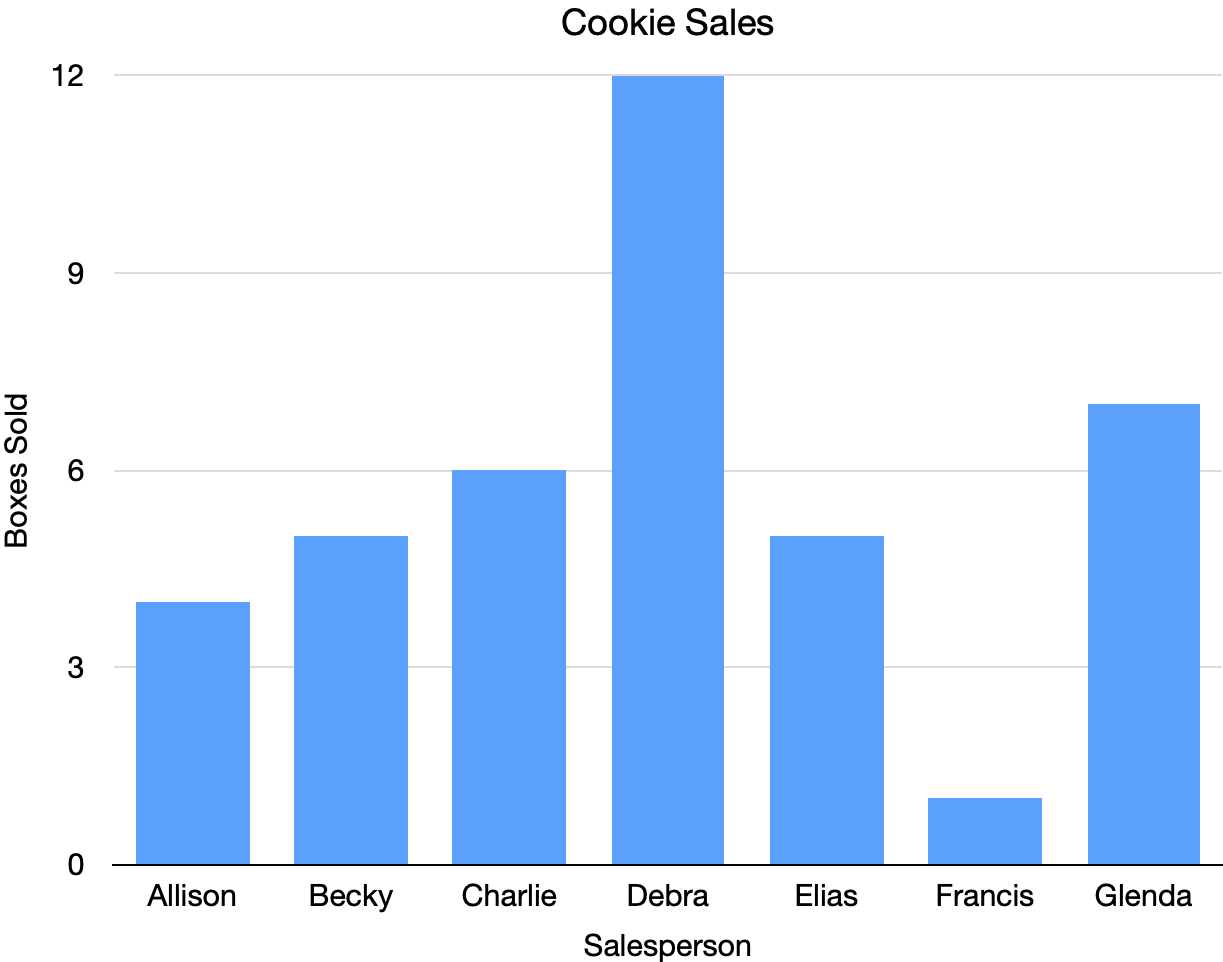
\includegraphics[width=0.7\textwidth]{CookieChart.png}
    \caption{A bar chart showing cookie sales per person.}
    \label{fig:bar}
\end{figure}

Each bar represents the cookie sales of one person. For example,
Charlie has sold 6 boxes of cookies, so the bar goes over Charlie's
name and reaches to the number 6.

Looking at this chart, you probably think, ``Wow, Debra has sold a lot
more cookies than anyone else, and Francis has sold a lot fewer.''

The same data could be in a table like this:

\begin{center}
  \begin{tabular}{c | c}
    Salesperson & Boxes Sold \\
    \hline
    Allison & 4 \\
    Becky & 5 \\
    Charlie & 6\\
    Debra & 12\\
    Elias & 5\\
    Francis & 1\\
    Glenda & 7
  \end{tabular}
\end{center}

A table (especially a large table) is often just a bunch of
numbers. A chart helps our brains understand what the numbers mean.

Bar charts can also go horizontally.
\begin{figure}[htbp]
    \centering
    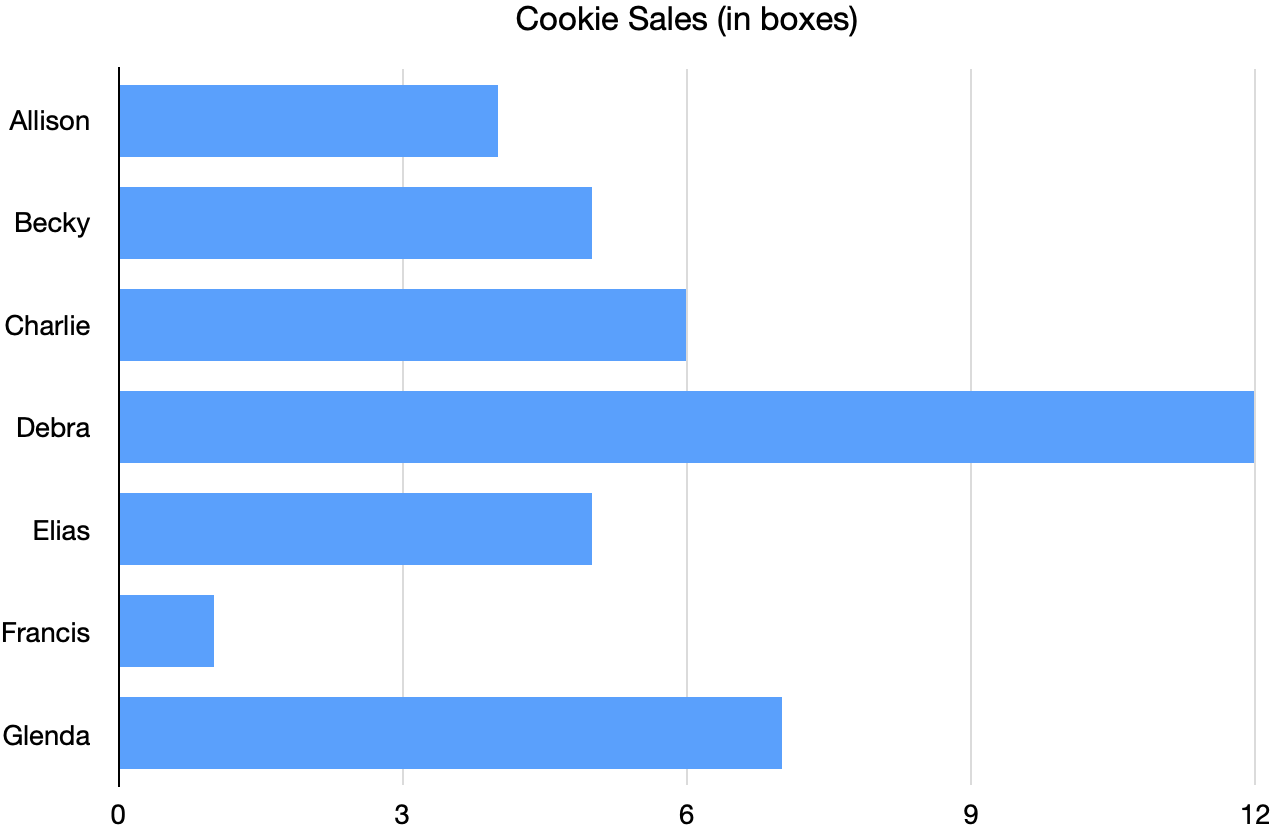
\includegraphics[width=0.7\textwidth]{HorizontalBarCookies.png}
    \caption{A horizontal bar chart showing the same cookie sales data.}
    \label{fig:horizontalBar}
\end{figure}

Sometimes we use colors to explain what contributed to the number.
\begin{figure}[htbp]
    \centering
    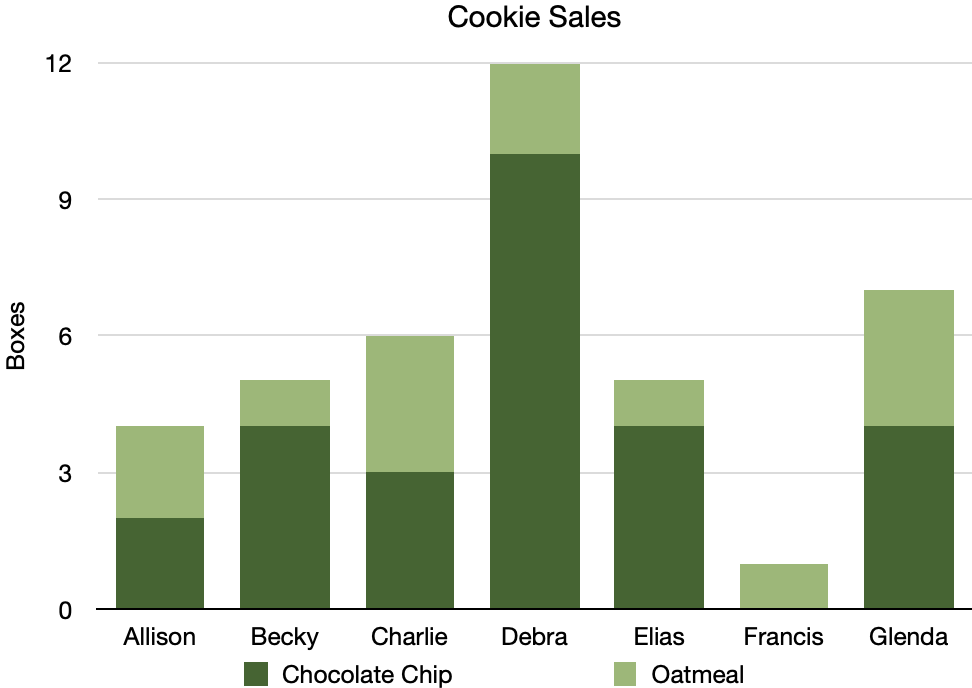
\includegraphics[width=0.7\textwidth]{TypesCookieBar.png}
    \caption{A bar chart with different colors showing types of cookes.}
    \label{fig:coloredBar}
\end{figure}

This tells us that Becky sold more boxes of chocolate chip cookies
than boxes of oatmeal cookies.

\subsection{Line Graph}

Here is a line graph:\index{line graph}
\begin{figure}[htbp]
    \centering
    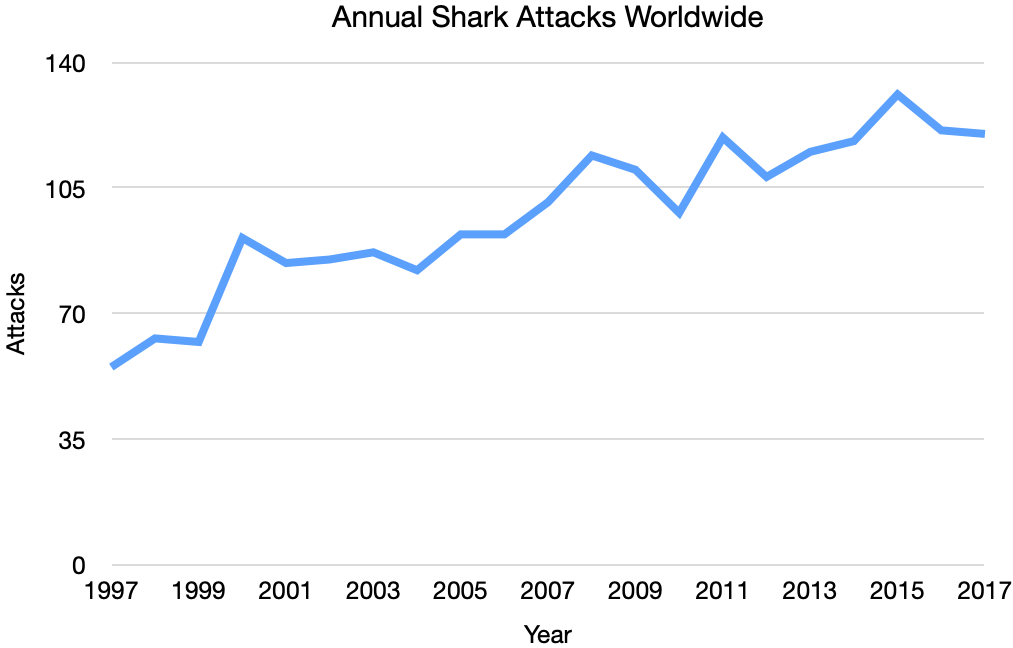
\includegraphics[width=0.7\textwidth]{SharksLine1.png}
    \caption{A line graph showing shark attacks per year over two decades.}
    \label{fig:lineSharkAttack}
\end{figure}

These are often used to show trends over time. Here, for example, you
can see that the number of shark attacks has been increasing over
time.

You can have more than one line on a graph.
\begin{figure}[htbp]
    \centering
    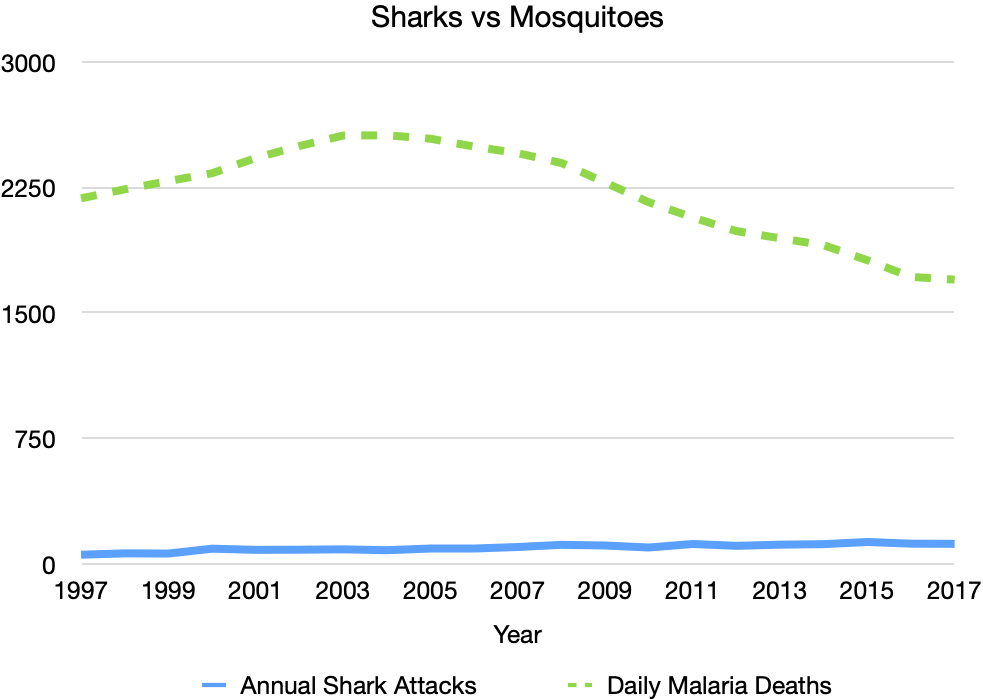
\includegraphics[width=0.7\textwidth]{SharksVsMosquitoes.png}
    \caption{A line graph showing shark deaths versus mosquito deaths.}
    \label{fig:lineSharkVsMosquito}
\end{figure}

\subsection{Pie Chart}

You use a pie chart when you are looking at the comparative size of numbers.\index{pie chart}
This is best for comparing percentages of a whole that sum to $100\%$. Here we can see that Nitrogen makes up $78\%$ of the gases in the air.
\begin{figure}[htbp]
    \centering
    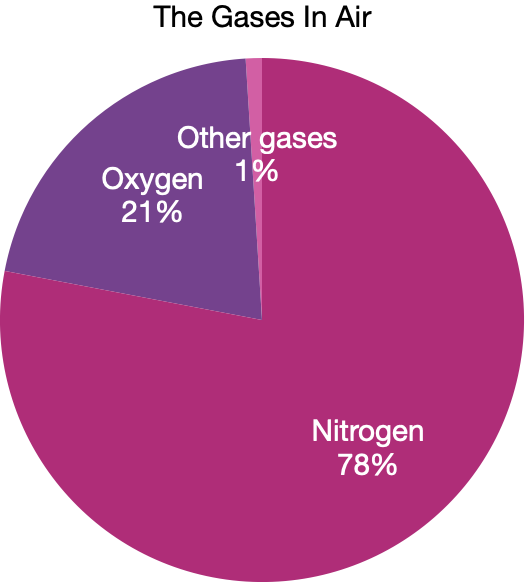
\includegraphics[width=0.4\textwidth]{AirPie.png}
    \caption{A pie chart of the various gases in the air.}
    \label{fig:AirPie}
\end{figure}

\subsection{Scatter Plot}

Sometimes, you have a large number of data points with two values, and you are
looking for a relationship between them.  For example, maybe you write
down the average temperature and the total sales for your lemonade
stand on the 15th of every month:\index{scatter plot}

\begin{center}
  \begin{tabular}{c | c | c}
    Date &	Avg. Temp. &	Total Sales \\
    \hline
  15 January 2022 & 2.6º C & \$183.85 \\
  15 February 2022 & -4.2º C & \$173.56\\
  15 March 2022 & 13.3º C & \$195.22\\
  15 April 2022 & 26.2º C & \$207.61\\
  15 May 2022 & 27.5º C & \$210.88\\
  15 June 2022 & 31.3º C & \$214.18\\
  15 July 2022 & 33.5º C & \$215.23\\
  15 Aug 2022 & 41.7º C & \$224.07\\
  15 September 2022 & 20.7º C & \$198.94\\
  15 October 2022 & 17.2º C & \$196.10\\
  15 November 2022 & 1.7º C & \$185.10\\
  15 December 2022 & 0.2º C & \$188.70 \\
  \end{tabular}
\end{center}

You may wonder, "Do I sell more lemonade on hotter days?''

To figure this out, you might create a scatter plot.  For each day, you put a mark that
represents that temperature and the sales that day:
%FIXME the labels in this graph are somewhat hard to see in the pdf

\begin{figure}[htbp]
    \centering
    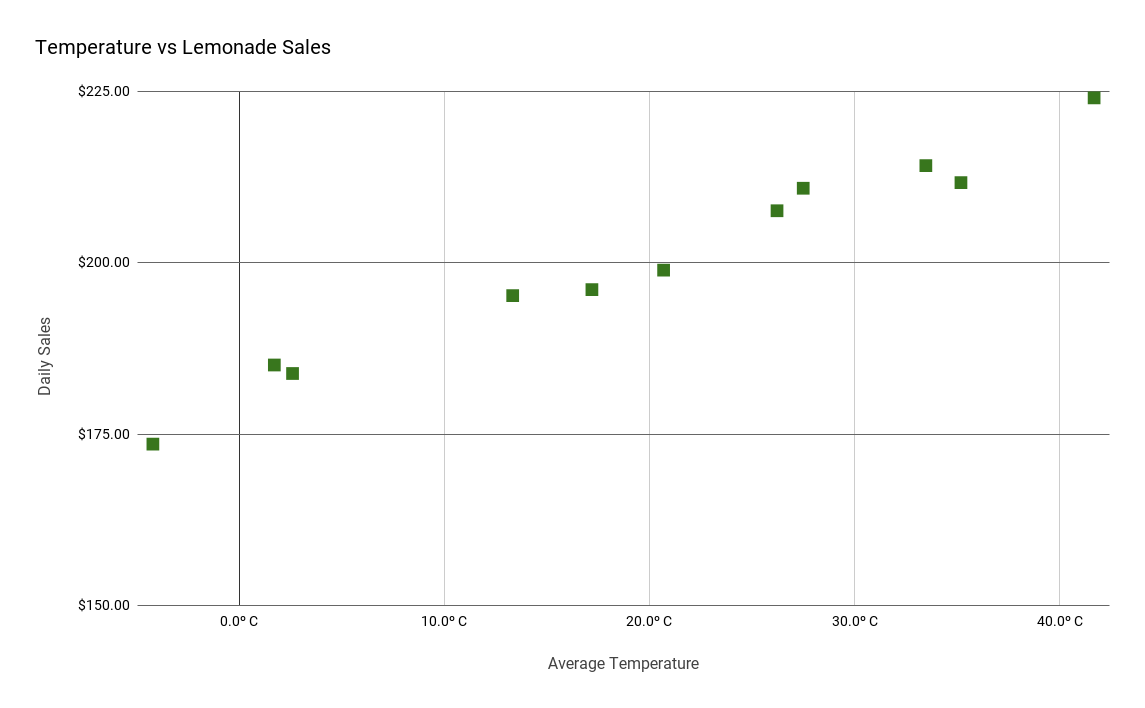
\includegraphics[width=\textwidth]{LemonadeScatter.png}
    \caption{A scatterplot of temperature versus daily sales.}
    \label{fig:scatterplot}
\end{figure}

From this scatter plot, you can easily see that you do sell more
lemonade as the temperature goes up. 
%FIXME diagram showing line of best fit
Drawing a \newterm{best-fit} line along the the points will give you a \newterm{correlation coefficient}. A positive correlation coefficient will give you a positively proportional relationship, while a negative coefficient will give you a inversely proportional relationship.

\section{Make Bar Graph}

Go back to your compound interest spreadsheet and make a bar graph
that shows both balances over time:
%FIXME this diagram is also hard to see
\begin{figure}[htbp]
    \centering
    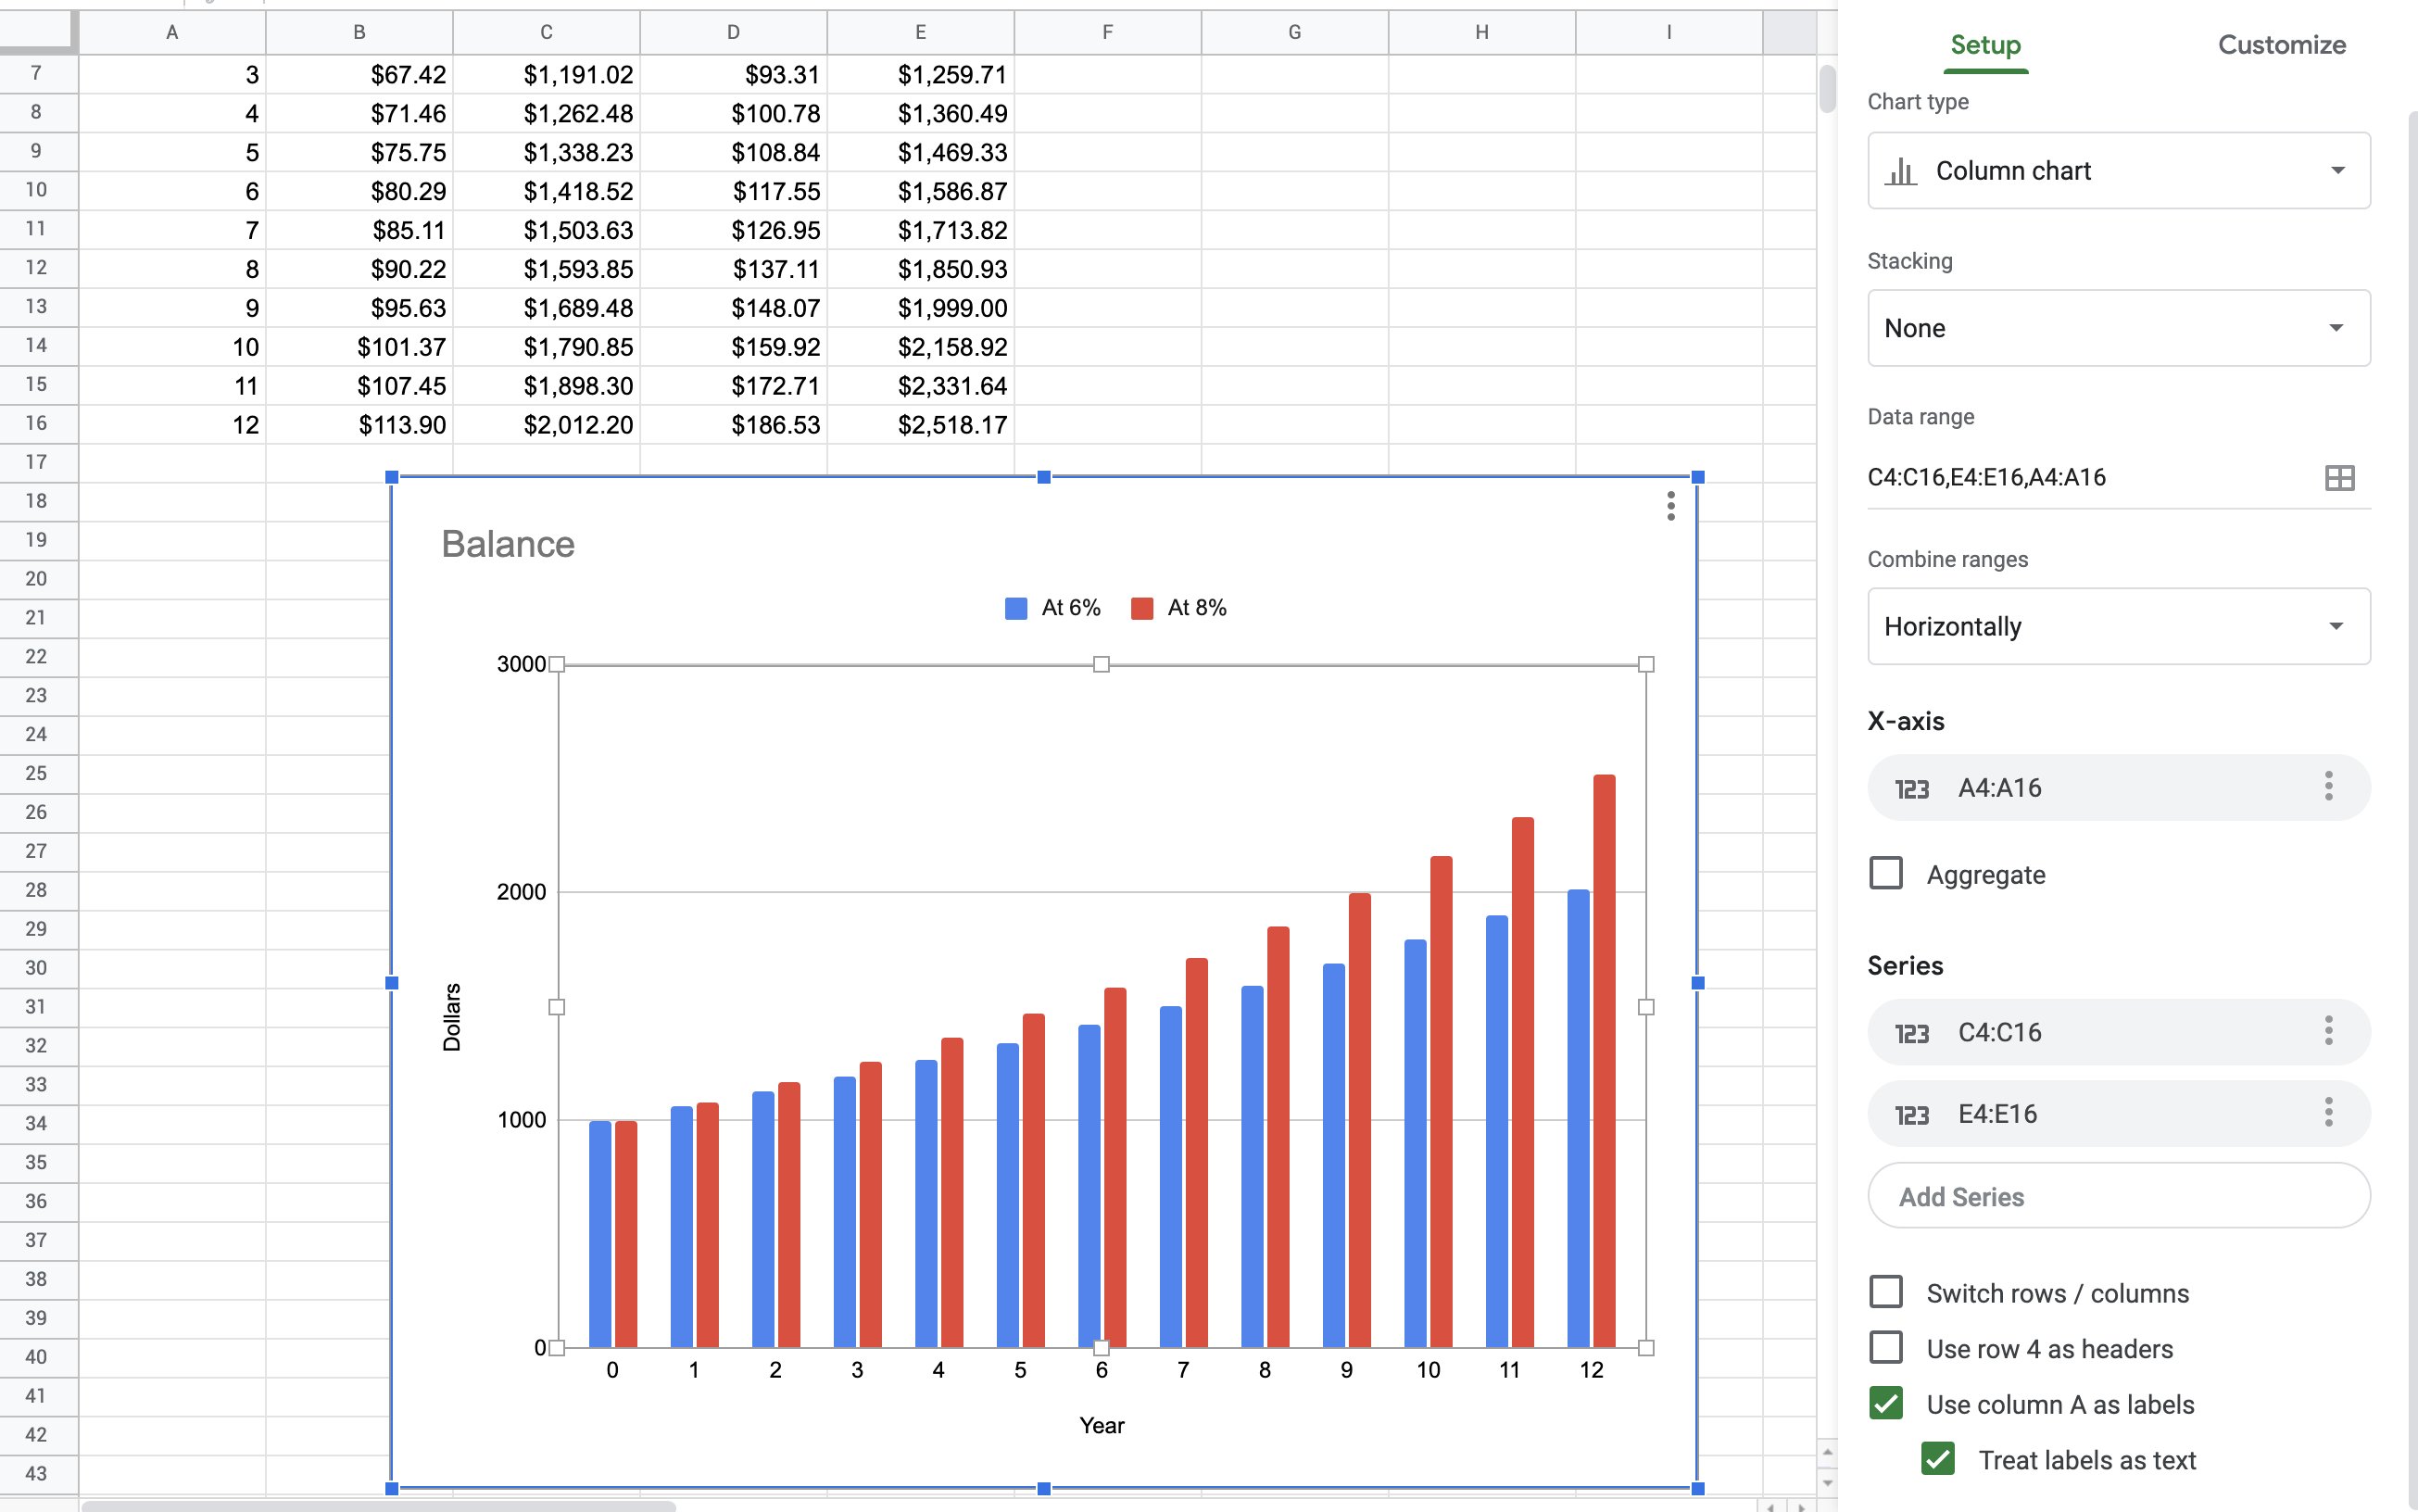
\includegraphics[width=0.9\textwidth]{InterestGraph.png}
    \caption{A bar graph made in google sheets showing interest.}
    \label{fig:spreadsheetBar}
\end{figure}

The year column should be used as the x-axis. There are two series of
data that come from C4:C16 and E4:E16.  Tidy up the titles and legend
as much as you like.\index{spreadsheet!graphing multiple series}

Looking at the graph, you can see the balances start the same, but
balance of the account with the larger interest rate quickly pulls
away from the account with the smaller interest rate.

